\documentclass[psamsfonts]{amsart}
\usepackage{amssymb,amsfonts}
\usepackage{enumerate}
\usepackage{mathrsfs}
\usepackage{mathtools}
\usepackage{algorithm}
\usepackage{algpseudocode}

\newcommand{\N}{\mathcal{N}}
\newcommand{\Bern}{\text{Bern}}

\title{Nested Sampling Comparisons}

\author{Won (Ryan) Lee}

%\date{October 1, 2015}

\begin{document}

%\begin{abstract}
%
%Give a brief description of your paper here
%
%\end{abstract}

\maketitle

%\tableofcontents

\section{Nested Sampling Algorithm}

This work compares the performance of the {\em nested sampling} algorithm proposed by Skilling \cite{skilling06} in computing the {\em evidence}, or marginal likelihood, of the data under a given model. We use an elementary version of the algorithm originally proposed in \cite{skilling06} and elaborated by Feroz et al. \cite{feroz14}, also referred to as the ``deterministic scheme" in Chopin and Robert \cite{chopin09} ({\bf Algorithm 1}):

\begin{algorithm}
\caption{Nested Sampling (Deterministic)}
\begin{algorithmic}
\State {\bf initialize}
\State $\Theta^i \sim \pi$ for $i =1, \dots, N$ independently
\State $\theta_1 = \arg\min_i L(\Theta^i) = \Theta^j$ for minimizing $j$
\State $Z = L(\theta_1) \cdot (1-e^{-1}/N)$
\While{$\max_i L(\Theta^i) e^{-t/N} > f \cdot Z$}
\State $\Theta^j \sim \pi|_{L(\theta) \geq L(\theta_t)}$ for $\theta_t = \Theta^j$ minimizing $L$ previously
\State $\theta_{t+1} = \arg\min_i L(\Theta^i)$
\State $Z = Z + L(\theta_{t+1})\cdot (e^{-t/N} - e^{-(t+1)/N})$
\EndWhile
\State $Z = Z + (N-1)^{-1} \sum_{i\neq j} L(\Theta^i) \cdot e^{-(t+1)/N}$
\State\Return $Z$, $\{\theta_t\}_{t\geq 1}$
\end{algorithmic}
\end{algorithm}

We note that the above scheme effectively fixes the unknown values of $x_t \equiv P(L(\theta) > L(\theta_t)$ as $x_t = e^{-t/N}$. The algorithm treats $L(\theta)$ as a random variable, and thus the values of $x_t$ are also stochastic. Thus, the ``deterministic" scheme above is contrasted in \cite{chopin09} with a ``random scheme" in which we initialize $x_{0,k} = 1$ for all $k = 1, \dots, K$, and at each iteration draw $K$ independent $r_{t,k} \sim \text{Beta}(N,1)$ and update the $x_{t,k} = x_{t-1,k} \cdot r_{t,k}$. \cite{chopin09} then suggest using the estimator:
$$\log Z \approx K^{-1} \sum_{k=1}^K \log Z_k$$
where $Z_k = \sum_t (x_{t+1,k} - x_{t,k})L(\theta_t)$ for each $k$. The authors note that for small values of $K$, this estimator produces more noisy estimates than the deterministic scheme (understandably) but may outperform the deterministic scheme if $K$ is large. The deterministic scheme is also the one explicitly proposed in \cite{skilling06}, with a note to sample the $x_t$ if desired to ``include its uncertainty."  This random scheme is given in {\bf Algorithm 2}.

For the restricted sampling step (or ``refreshment") $\Theta^j \sim \pi_{L(\theta) \geq L(\theta_t)}$, we use simple Monte Carlo sampling and resample as necessary to obtain some $\theta^* \sim \pi$, rejecting the proposed values until $L(\theta^*) \geq L(\theta_t)$. E. Cameron (and others) note that a random MCMC move can be used at this step, which may improve performance.

\begin{algorithm}
\caption{Nested Sampling (Random)}
\begin{algorithmic}
\State {\bf initialize}
\State $\Theta^i \sim \pi$ for $i =1, \dots, N$ independently
\State $\theta_1 = \arg\min_i L(\Theta^i) = \Theta^j$ for minimizing $j$
\State $x_{1,k} \sim \text{Beta}(N,1)$ for $k = 1, \dots, K$ independently
\State $Z_k = L(\theta_1) \cdot (1-x_{1,k})$
\While{$\max_i L(\Theta^i) e^{-t/N} > f \cdot \bar{Z}$}
\State $\Theta^j \sim \pi|_{L(\theta) \geq L(\theta_t)}$ for $\theta_t = \Theta^j$ minimizing $L$ previously (iteration $t$)
\State $\theta_{t+1} = \arg\min_i L(\Theta^i)$
\State $x_{t+1,k} = x_{t,k} \cdot r_{t+1,k}$ for $r_{t+1,k} \sim \text{Beta}(N,1)$ independently
\State $Z_k = Z_k + L(\theta_{t+1})\cdot (x_{t,k} - x_{t+1,k})$
\EndWhile
\State $Z_k = Z_k + (N-1)^{-1} \sum_{i\neq j} L(\Theta^i) \cdot e^{-(t+1)/N}$
\State $\log Z = K^{-1} \sum_{k=1}^K\log Z_k$
\State\Return $Z$, $\{\theta_t\}_{t\geq 1}$
\end{algorithmic}
\end{algorithm}

\section{Normal-Normal Conjugate Model}

We start by considering a Normal-Normal conjugate model. We consider a Normal prior: $\theta\sim\mathcal{N}(\mu,\tau^2)$, and $n$ observations $Y_1,\ldots,Y_n$ independently distributed as $Y_i|\theta\sim\mathcal{N}(\theta,\sigma^2)$.
The prior and the likelihood are conjugate so that we can compute exactly the moments of the posterior distributions.
Note also that we can compute the normalizing constant (also called the evidence) exactly. Indeed, the normalizing constant
$p(Y_{1}, Y_{2}, ... , Y_{n})$ satisfies
 \[
p(Y_{1}, Y_{2}, ... , Y_{n}) = p(Y_1) \prod_{i=2}^n p(Y_i| Y_1, \ldots, Y_{i-1}),
 \]
and each incremental evidence satisfies
 \[
 p(Y_i | Y_{1}, Y_{2}, ... , Y_{i-1}) = \int p(Y_i | \theta) p(\theta | Y_{1}, Y_{2}, ... , Y_{i-1}) d\theta.
 \]
 This integral has a closed-form solution in the Normal case, given by:
 \[
 \int\varphi_{\mathcal{N}}(x;\theta,\lambda)\varphi_{\mathcal{N}}(x;\mu_{i-1},\lambda_{i-1}) dx=\frac{1}{\sqrt{2\pi\left(\lambda^{-1}+\lambda_{i-1}^{-1}\right)}}\exp\left(-\frac{1}{2\left(\lambda^{-1}+\lambda_{i-1}^{-1}\right)}\left(y_i-\mu_{i-1}\right)^{2}\right).
 \]
 where $\varphi_{\mathcal{N}}(x;\mu,\lambda)$ denotes the Normal density evaluated at $x$, with mean $\mu$ and precision $\lambda$ (that is, one over the variance). Then we have $\lambda = \tau^{-2}$ and $\lambda' = \sigma^{-2}$. The posterior:
 $$\theta|Y_1, \dots, Y_i \sim \mathcal{N}\left( \frac{i\bar{y}_i\lambda'}{\lambda' + i\lambda}, \frac{1}{\lambda' + i\lambda} \right) $$
 suggests that we define:
 $$\lambda_i = \tau^{-2} + i\sigma^{-2} = \lambda + i\lambda'$$
 $$\mu_i = \frac{n \bar{y} \lambda'}{\lambda_i}$$
 Thus, the incremental evidence satisfies:
 $$Y_i|Y_1,\dots,Y_{i-1} \sim \mathcal{N}(\mu_{i-1}, \lambda^{-1} + \lambda_{i-1}^{-1})$$  
 
 \subsection{Importance Sampling Comparison}
 
 We first compare the algorithm to a sequential importance sampling (SIS) scheme in which the particles are drawn from a $\mathcal{N}(0,1)$ prior, and the data are also generated $Y_1, \dots, Y_n \sim \mathcal{N}(0,1)$ independently (i.e. the ideal situation for SIS to be effective). Noting that the above decomposition of the evidence yields a log decomposition:
 $$\log Z = \log p(Y_1) + \sum_{i=2}^n \log p(Y_i|Y_1, \dots, Y_{i-1})$$
We consider the computation of the weights:
$$w_k(\Theta^i) = w_{k-1}(\Theta^i)\frac{\pi_{u,k}(\Theta^i)}{\pi_{u,k-1}(\Theta^i)} = w_{k-1}(\Theta^i) \frac{\mathcal{L}_{1:k}(\Theta^i)\pi(\Theta^i)}{\mathcal{L}_{1:k-1}(\Theta^i)\pi(\Theta^i)}$$
where $\mathcal{L}_{1:k}(\Theta) \equiv \prod_{i=1}^k p(y_i|\Theta)$ by independence, we see that this simplifies to:
$$w_k(\Theta^i) = w_{k-1}(\Theta^i)p(y_k|\Theta^i)$$
so that in log-weights:
$$\log w_k(\Theta^i) = \log w_{k-1}(\Theta^i) + \log \mathcal{L}_k (\Theta^i)$$

This allows for the sequential computation of evidence at each data point $Y_k$, as:
$$Z_k \equiv p(Y_1, \dots, Y_k) \approx \frac{1}{N} \sum_{i=1}^N w_k (\Theta^i)$$
where each $\log w_k(\Theta^i)$ can be computed sequentially as above.

We have a number of parameters to tune for each algorithm. For importance sampling, we must set $N$, the number of $\Theta$ particles; for nested sampling, we must set both $N$, which is now the number of alive $\Theta$ particles in any iteration, as well as $f$, the threshold of the current evidence at which to terminate, i.e. terminate the algorithm when:
$$\max \mathcal{L}(\Theta^i) e^{-t/N} \leq f\cdot Z_t$$
where $t$ is the current iteration and $Z_t$ is the evidence cumulatively summed to that iteration. (That is, we terminate the algorithm when the next increment added to the total evidence is less than $f$ of the cumulative evidence up to that iteration.)

We vary both parameters. We let $n = 100$ be the number of observations $Y_i$ and do 100 runs of each simulation. Moreover, $N$ is set to be equal in each run for both the IS and NS samplers for sake of comparison. Figures and tables follow:\\

%\begin{table}[b]\centering
%\begin{tabular}{c|c|c|c|c|c}
%$f$ & $N$ & IS Evidence & IS Variance & NS Evidence & NS Variance \\\hline
%0.01 & 100 &  -138.793 &0.05595  & -138.802 & 0.02115\\
%0.01 & 1000 & -138.781 & 0.005535 & -138.799 & 0.001884\\
%0.05 & 1000 &-138.779 & 0.004806 & -138.830 & 0.001779\\
%0.01 & 10000 & -138.782 & 0.00056 & -138.831 & 0.00018\\
%\end{tabular}\\
%\caption{Comparison of IS and NS-det samplers for computing $\log Z$, the evidence, for a Normal-Normal conjugate model with varying parameters. The values are in log, and the exact log-evidence was -138.783.}
%\end{table}

\begin{table}\centering
\caption{Comparison of IS, NS-det, and NS-rand samplers for computing $\log Z$ for 100 particles and $f = 0.01$ over 100 runs; the NS-rand sampler is run with 100 parallel quadrature points given by $x_{t,k} = x_{t-1,k} \cdot r_{t,k}$ for $r_{t,k} \sim \text{Beta}(N,1)$.}
\begin{tabular}{c|c|c|c}
Exact Evidence & IS Mean & IS Var & IS RMSE\\\hline
-130.480 & -130.524 & 0.0609 & 0.04518 \\
& & & \\
NS-det Iterations  & NS-det Mean & NS-det Var & NS-det RMSE \\\hline
690.6 & -130.463 & 0.0213 & 0.0173\\
& & & \\
NS-rand Iterations & NS-rand Mean & NS-rand Var & NS-rand RMSE \\\hline
692.8 & -130.483 & 0.0160  & 0.000645 \\
\end{tabular}\\

\end{table}

\begin{table}\centering
\caption{Comparison of IS, NS-det, and NS-rand samplers in mean and RMSE for computing $\log Z$ for differing numbers of particles ($N = 100, 1000, 10000$) with the same threshold ($f = 0.01$). The exact log-evidence value was $\log Z = -130.48$.}
\begin{tabular}{c|c|c|c|c|c|c}
N & IS & NS-det & NS-rand & IS RMSE & NS-det RMSE & NS-rand RMSE \\\hline
100 &-130.52 & -130.46 & -130.48 & 0.248 & 0.146 & 0.127\\
1000 & -130.47 & -130.49 & -130.49 & 0.0802 & 0.0401 & 0.0094 \\
10000 & -130.48 & -130.49 & -130.49 & 0.022 & 0.0167 & 0.0163\\

\end{tabular}\\



\end{table}

\subsection{Results}

In general, it appears that the NS sampler yields lower variance than the corresponding IS sampler in evidence estimates. Both samplers do quite well in estimating the evidence, with the IS sampler more or less uniformly dominating in terms of mean estimates over 100 runs. Interestingly, the NS sampler appears to become progressively biased (which is most clearly illustrated in Figure 3) as $N$, the number of alive particles, increases. Given that the bias is negative, it appears that having a higher $N$ yields a more fine-grained sample of $\Theta^i$ and consequent early termination of the algorithm. This is also unintuitive, however, as a higher number of alive particles should yield higher probabilities of the particles being closer to the maximum likelihood value.

\begin{figure}
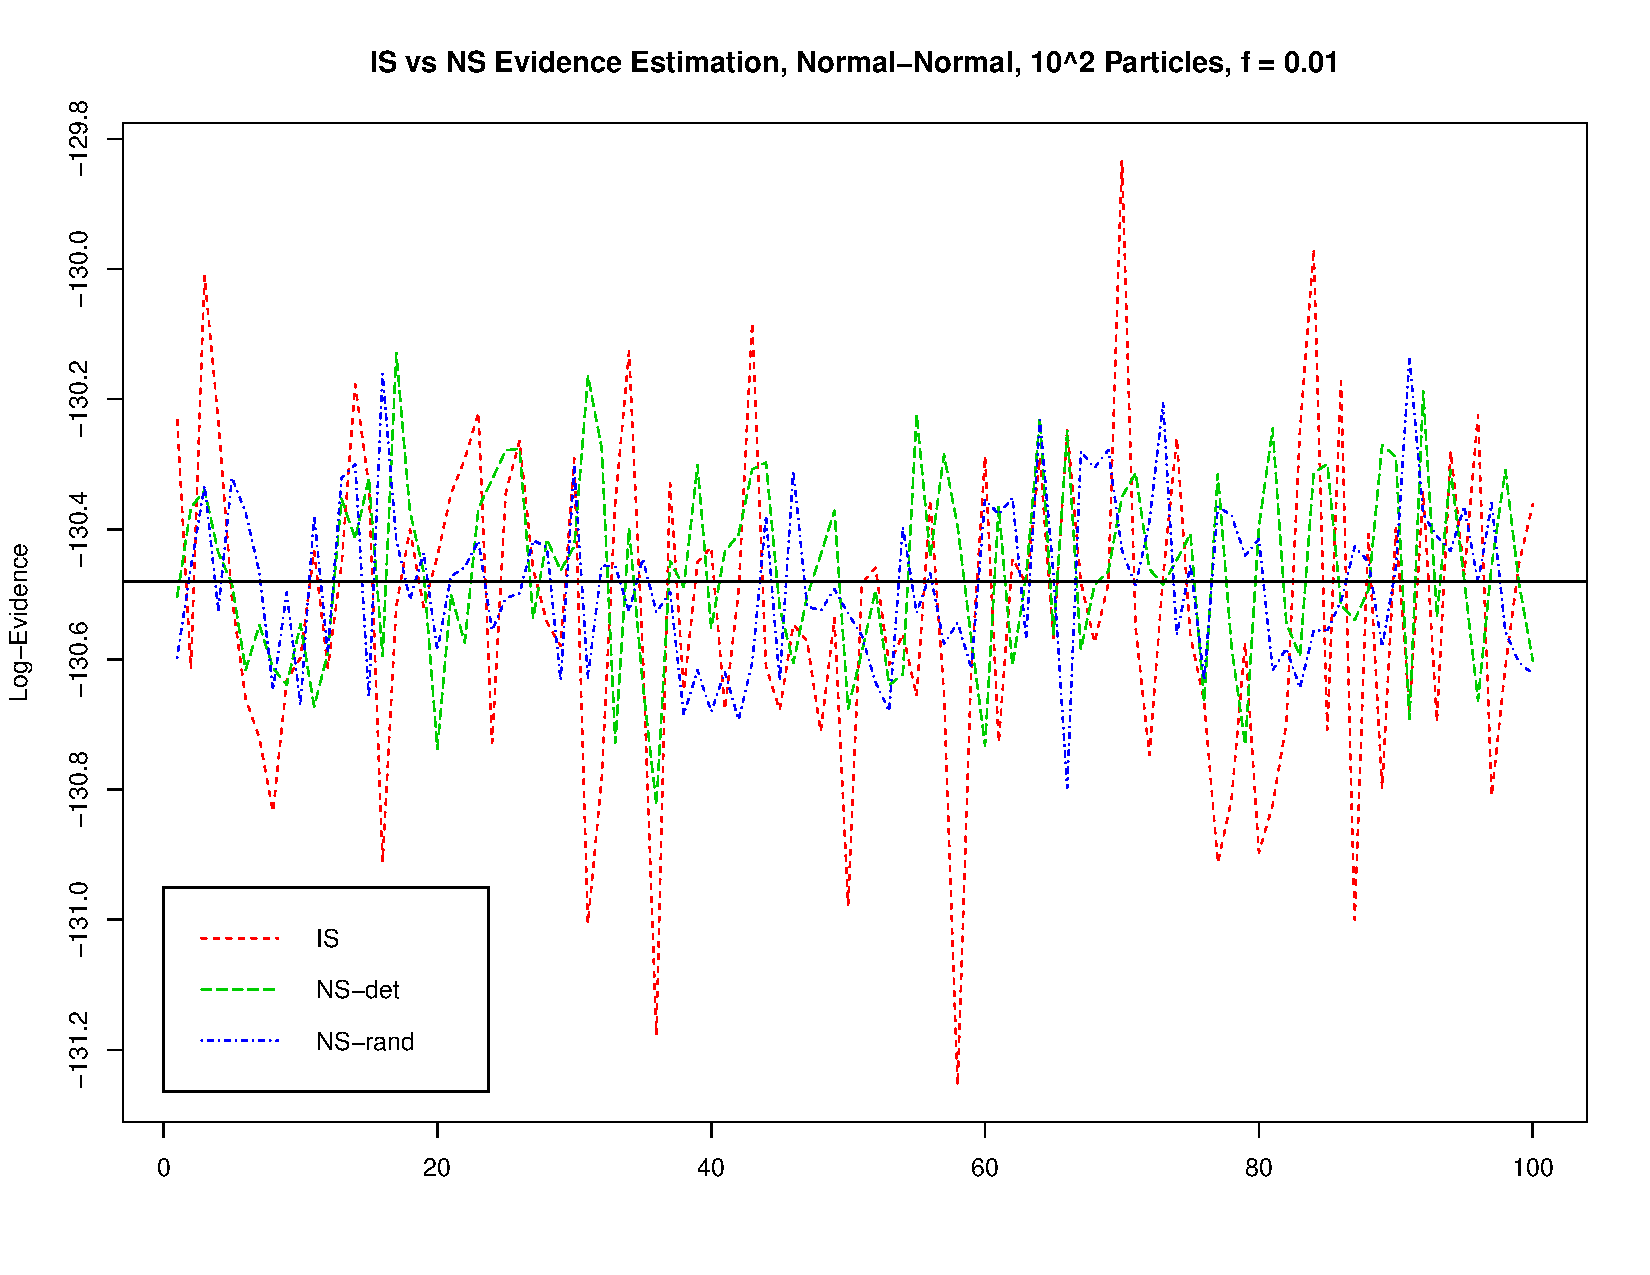
\includegraphics[width=0.7\textwidth]{N-N_10e2_f01_rand.pdf}

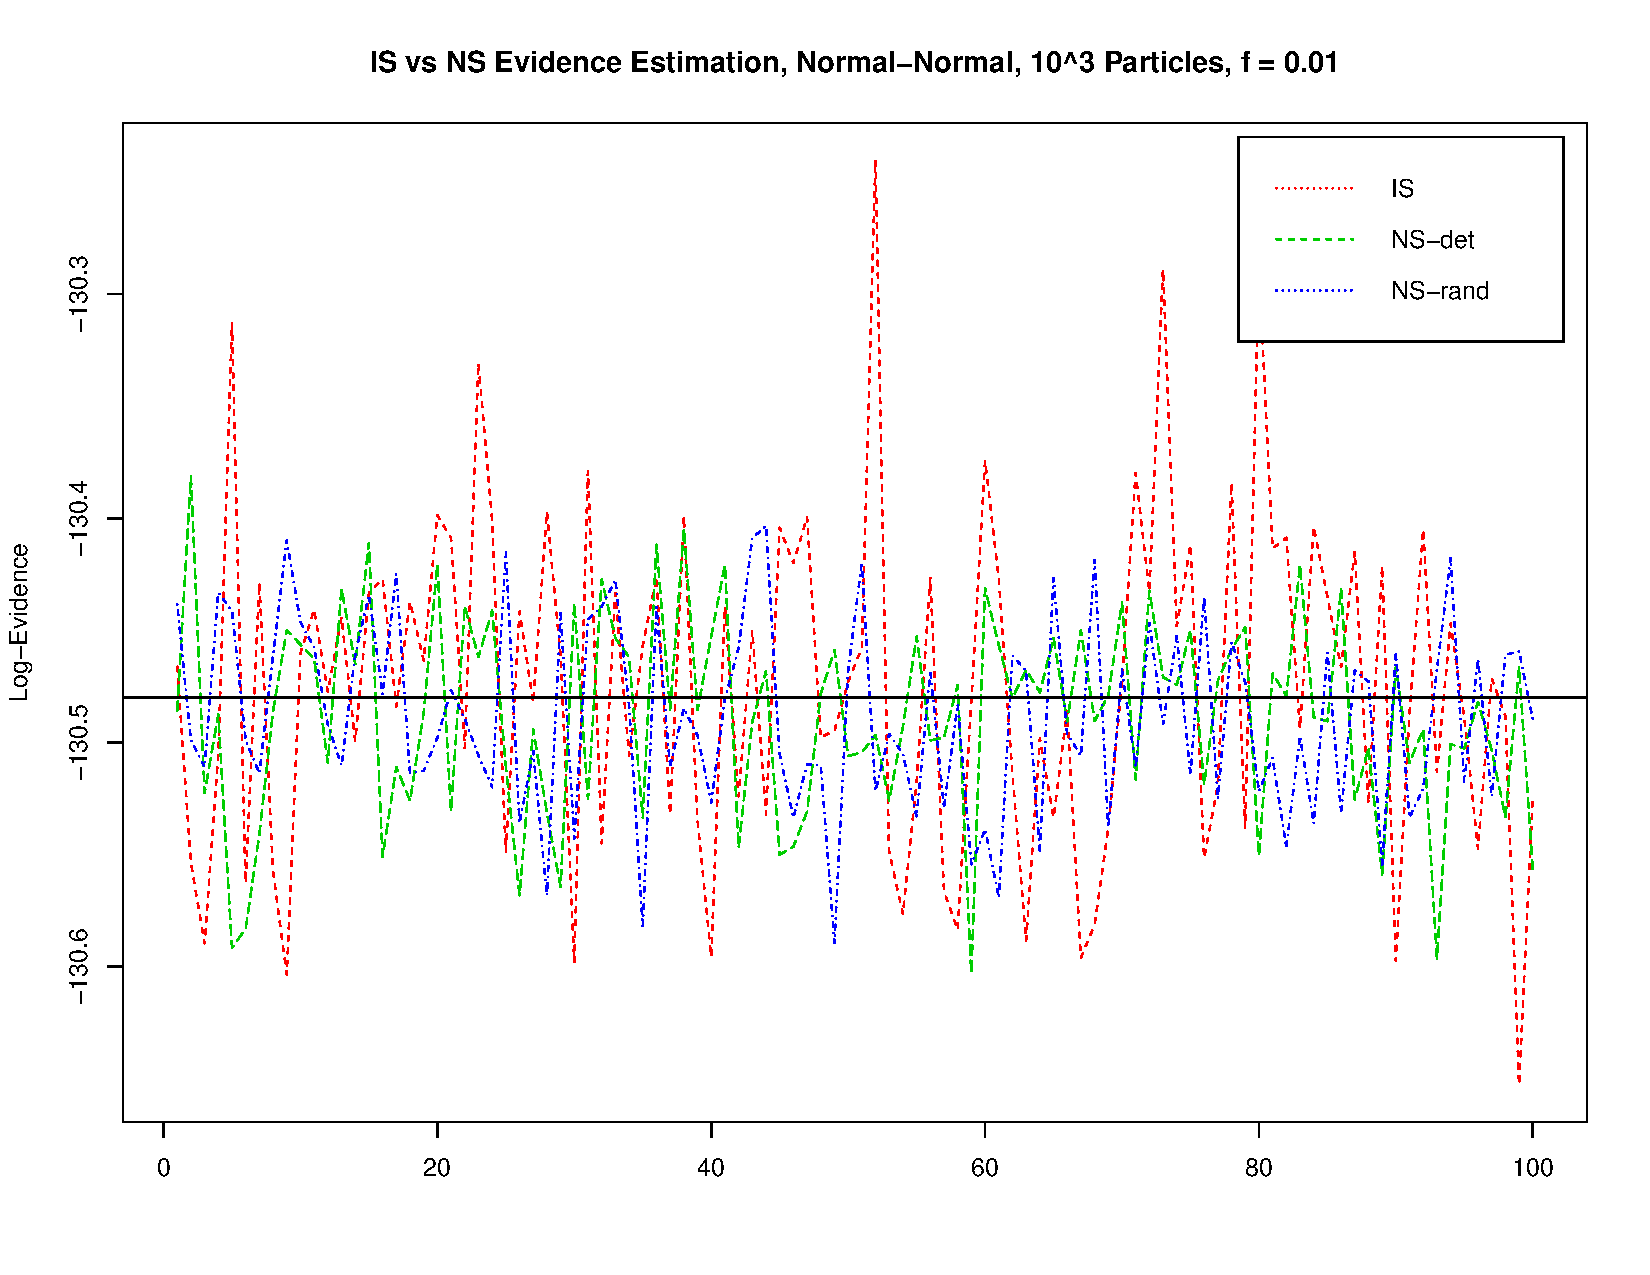
\includegraphics[width=0.7\textwidth]{N-N_10e3_f01_rand.pdf}

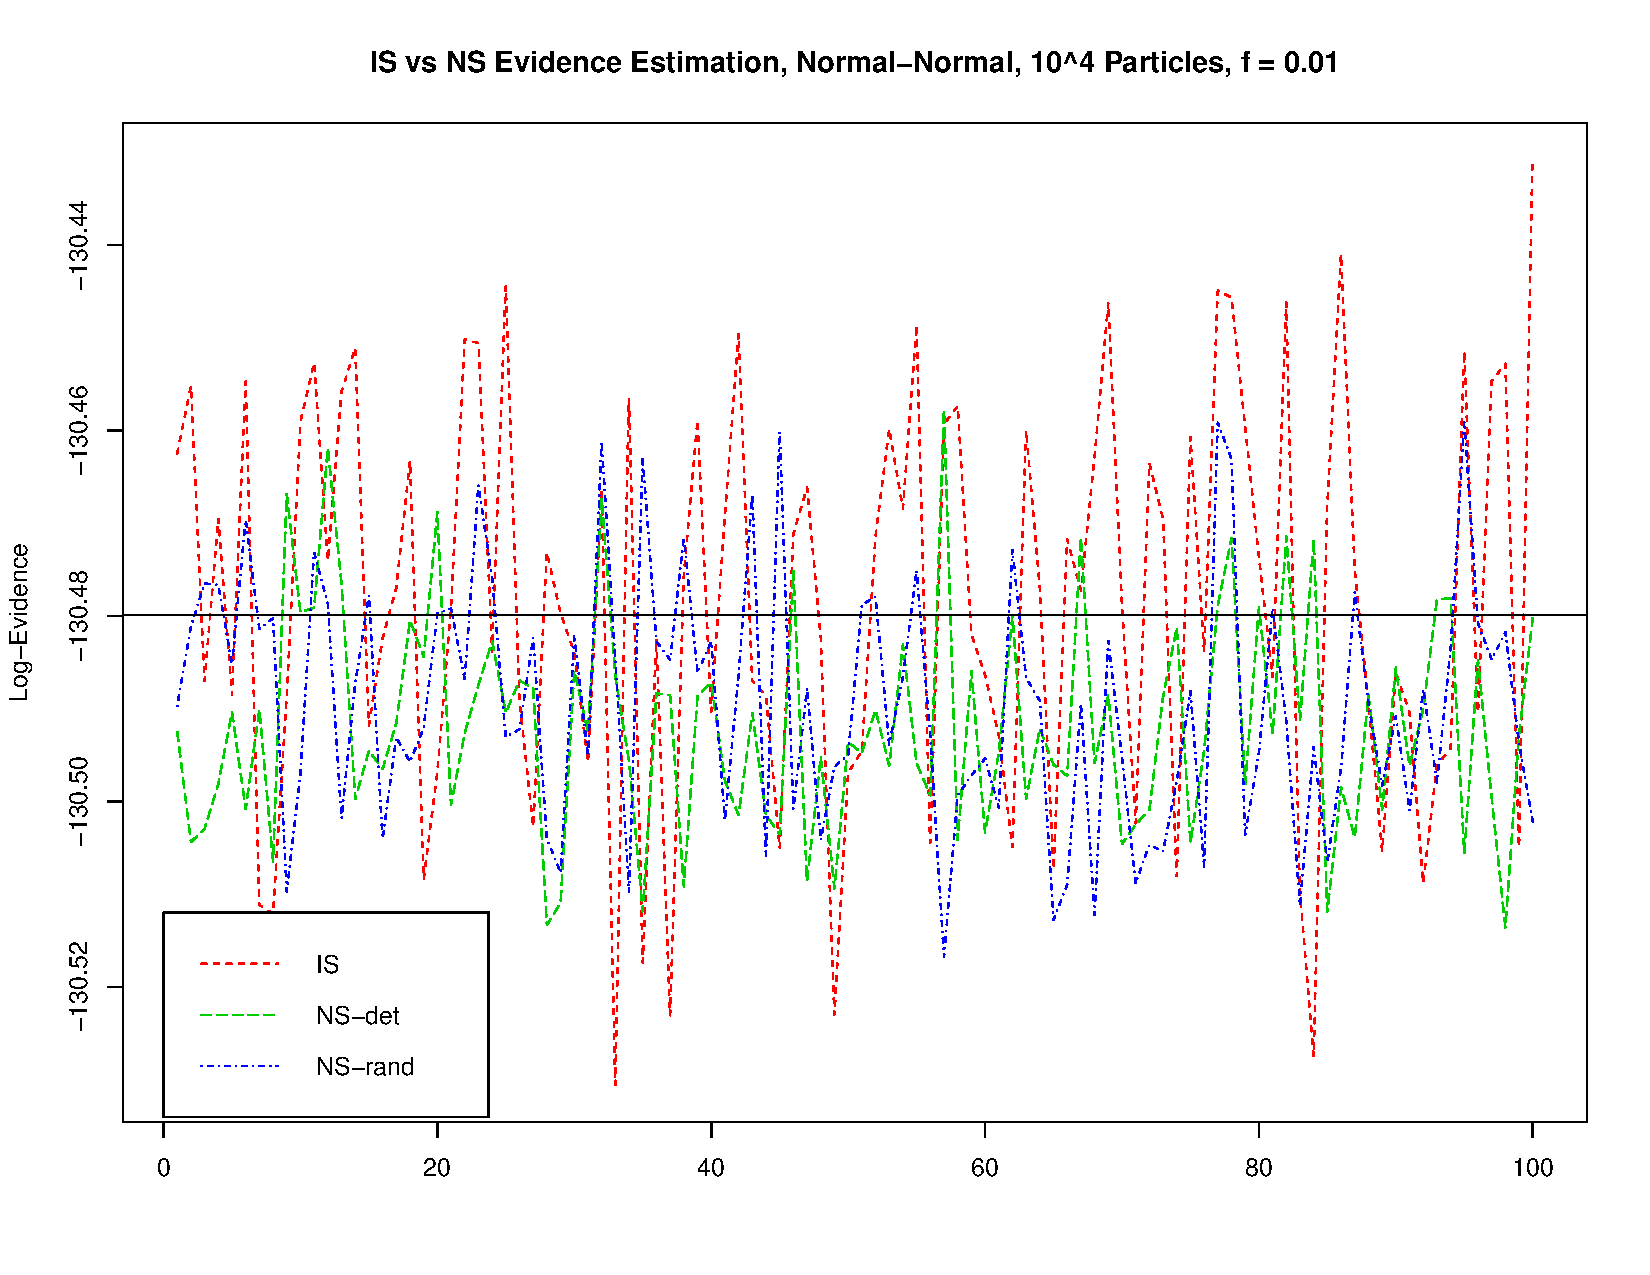
\includegraphics[width=0.7\textwidth]{N-N_10e4_f01_rand.pdf}

\caption{Comparison of log-evidence estimates for the Normal-Normal conjugate model using the SIS, NS-det, and NS-rand samplers and varying numbers of particles $N = 100, 1000, 10000$.}
\end{figure}



\section{Two Normal Mixture Model}

In this section, we consider the following (hierarchical) mixture model with varying degrees of complexity:
$$\lambda \sim \text{Bern}(p)$$
$$\mu_i \sim \mathcal{N}(\theta, \tau^2)$$
$$y|\lambda = i, \mu_i, \sigma_i^2 \sim \mathcal{N}(\mu_i, \sigma_i^2)$$

\subsection{Known Parameters}

At first, we consider no hyperdistribution on $\mu_i, \sigma_i^2$, considering them to be known, fixed constants. The simplest case is one in which we assume that $p = 1/2$ is fixed, and we are simply computing the evidence $p(y) \equiv p(y_1, \dots, y_n)$ knowing all model parameters but oblivious to the values of the latent $\lambda_i$ for each $y_i$. Even for this simple case, for any reasonable number of observations $n$, the computations require consideration of every possible configuration ($2^{100}$ possibilities) for the $\lambda_i$. 

\subsection{Means Unknown, Variances Known}

We now generalize and consider the $\mu_i \sim \mathcal{N}(\theta, \tau^2)$ to be drawn i.i.d. from a Normal hyperdistribution with parameters $\theta, \tau^2$. We again consider $\lambda$ to be latent, unknown variables drawn from $\text{Bern}(1/2)$. Again, the exact computations for the evidence are intractable, so we resort to an ``exact" Monte Carlo estimate of the evidence as follows:
\begin{align*}
p(y) &= \int p(y|\lambda, \mu_1, \mu_2) p(\lambda, \mu_1, \mu_2) d\lambda d\mu_1 d\mu_2 \\
&= \int \left[ \int p(y|\lambda, \mu_1,\mu_2)p(\mu_1)p(\mu_2) d\mu_1 d\mu_2\right] p(\lambda) d\lambda
\end{align*}

We can compute the inner integral analytically for any configuration of the latent $\lambda$, and then draw $\lambda$ i.i.d. $\text{Bern}(1/2)$, evaluate the inner integral at the sample values of $\lambda$, then take the average to obtain a Monte Carlo estimate.

For sake of simplicity, we take $\sigma_1^2 = \sigma_2^2 = \sigma^2$ to be known and fixed throughout the calculation. By conjugacy, we can compute the integral analytically as follows:
\begin{align*}
p(y|\lambda, &\mu_1,\mu_2)p(\mu_1)p(\mu_2)  \\
=& \prod_{i=1}^n \N(y_i|\mu_{\lambda_i}, \sigma^2) \N(\mu_1|\theta, \tau^2)\N(\mu_2|\theta, \tau^2)\\
=& \left[ \prod_{\lambda_i = 1} \N(y_i|\mu_1, \sigma^2)\right] \left[ \prod_{\lambda_i = 2} \N(y_i|\mu_2, \sigma^2) \right] \N(\mu_1|\theta,\tau^2)\N(\mu_2|\theta,\tau^2)\\
=& (2\pi\sigma^2)^{-n/2} (2\pi\tau^2)^{-1} \exp\left[ -\frac{1}{2\sigma^2}\left( \sum_{\lambda_i = 1} y_i^2 - n_1\bar{y}_1^2\right) - \frac{n_1}{2\sigma^2} (\mu_1-\bar{y}_1)^2\right.\\
&- \left.\frac{1}{2\sigma^2}\left(\sum_{\lambda_i = 2}y_i^2 - n_2\bar{y}_2^2\right) - \frac{n_2}{2\sigma^2}(\mu_2-\bar{y}_2)^2 - \frac{1}{2\tau^2}(\mu_1-\theta)^2 - \frac{1}{2\tau^2}(\mu_2 -\theta)^2\right]
\end{align*}
where the third line follows by completing squares. Expanding out in the $\mu_i$ and completing squares again yields the expression:
\begin{align*}
p(y|\lambda, &\mu_1,\mu_2)p(\mu_1)p(\mu_2) \\
=& (2\pi\sigma^2)^{-n/2} (2\pi\tau^2)^{-1} \exp\left[ -\frac{1}{2\sigma^2}\left( \sum_{\lambda_i = 1} y_i^2 - n_1\bar{y}_1^2 \sum_{\lambda_i = 2}y_i^2 - n_2\bar{y}_2^2 \right)\right.\\ 
&- \left.\left( \frac{n_1}{2\sigma^2} \bar{y}_1^2 + \frac{1}{2\tau^2}\theta^2 + \frac{n_2}{2\sigma^2} \bar{y}_2^2 + \frac{1}{2\tau^2} \theta^2\right) + \left(\frac{n_1}{2\sigma^2} + \frac{1}{2\tau^2} \right) \tilde{\mu}_1^2 + \left(\frac{n_2}{2\sigma^2} + \frac{1}{2\tau^2}\right)\tilde{\mu}_2^2 \right]\\
& \times \exp\left[-\frac{1}{2}(n_1/\sigma^2 + 1/\tau^2) (\mu_1-\tilde{\mu}_1)^2\right] \exp\left[-\frac{1}{2}(n_2/\sigma^2 + 1/\tau^2) (\mu_2 - \tilde{\mu}_2)^2\right] 
\end{align*}
where we have:
$$\tilde{\mu}_i \equiv \frac{\frac{n_i\bar{y}_i}{2\sigma^2} + \frac{\theta}{2\tau^2}}{\frac{n_i}{2\sigma^2} + \frac{1}{2\tau^2}}$$
Finally, integrating out $\mu_1, \mu_2$ in the density yields the inner integral:
\begin{align*}
\int p(y|\lambda, &\mu_1,\mu_2)p(\mu_1)p(\mu_2) d\mu_1 d\mu_2 \\
&= (2\pi\sigma^2)^{-n/2} (2\pi\tau^2)^{-1} \exp\left[ -\frac{1}{2\sigma^2}\left( \sum_{\lambda_i = 1} y_i^2 - n_1\bar{y}_1^2 \sum_{\lambda_i = 2}y_i^2 - n_2\bar{y}_2^2 \right)\right.\\ 
&- \left.\left( \frac{n_1}{2\sigma^2} \bar{y}_1^2 + \frac{1}{2\tau^2}\theta^2 + \frac{n_2}{2\sigma^2} \bar{y}_2^2 + \frac{1}{2\tau^2} \theta^2\right) + \left(\frac{n_1}{2\sigma^2} + \frac{1}{2\tau^2} \right) \tilde{\mu}_1^2 + \left(\frac{n_2}{2\sigma^2} + \frac{1}{2\tau^2}\right)\tilde{\mu}_2^2 \right]\\
&\times \left(\frac{2\pi}{n_1/\sigma^2 + 1/\tau^2}\right)^{-1/2}\left(\frac{2\pi}{n_2/\sigma^2+1/\tau^2}\right)^{-1/2} 
\end{align*}

Again, computing the above integral at sample values of $\lambda$ and averaging the results yields an ``exact" Monte Carlo estimate of the evidence.

For the computation of the evidence by SIS or NS, we sample the particles:
$$\Theta^i = (\lambda^i, \mu_1^i, \mu_2^i) \sim \Bern(1/2)\cdot\N(\mu_1|\theta,\tau^2)\cdot\N(\mu_2|\theta, \tau^2)$$
and follow the algorithms above as before.

\subsection{Results} Because of the multidimensionality of the parameter space $\Theta = \Lambda\times\mathbb{R}\times\mathbb{R}$, the SIS algorithm fares rather poorly in this example, particularly compared to the ideal Normal-Normal previously. As seen in {\bf Figure 2}, the effective sample size (ESS) decreases uniformly to below 5 (out of $N = 100$ particles) after approximately half the observations have been incorporated, with most runs falling to the minimum of $ESS = 1$ very quickly. This indicates that estimation is based on only a few $< 5$ particles $\Theta^i$, which results in the relatively poor performance and large variance of the log-evidence estimates using SIS in this model.

\begin{figure}
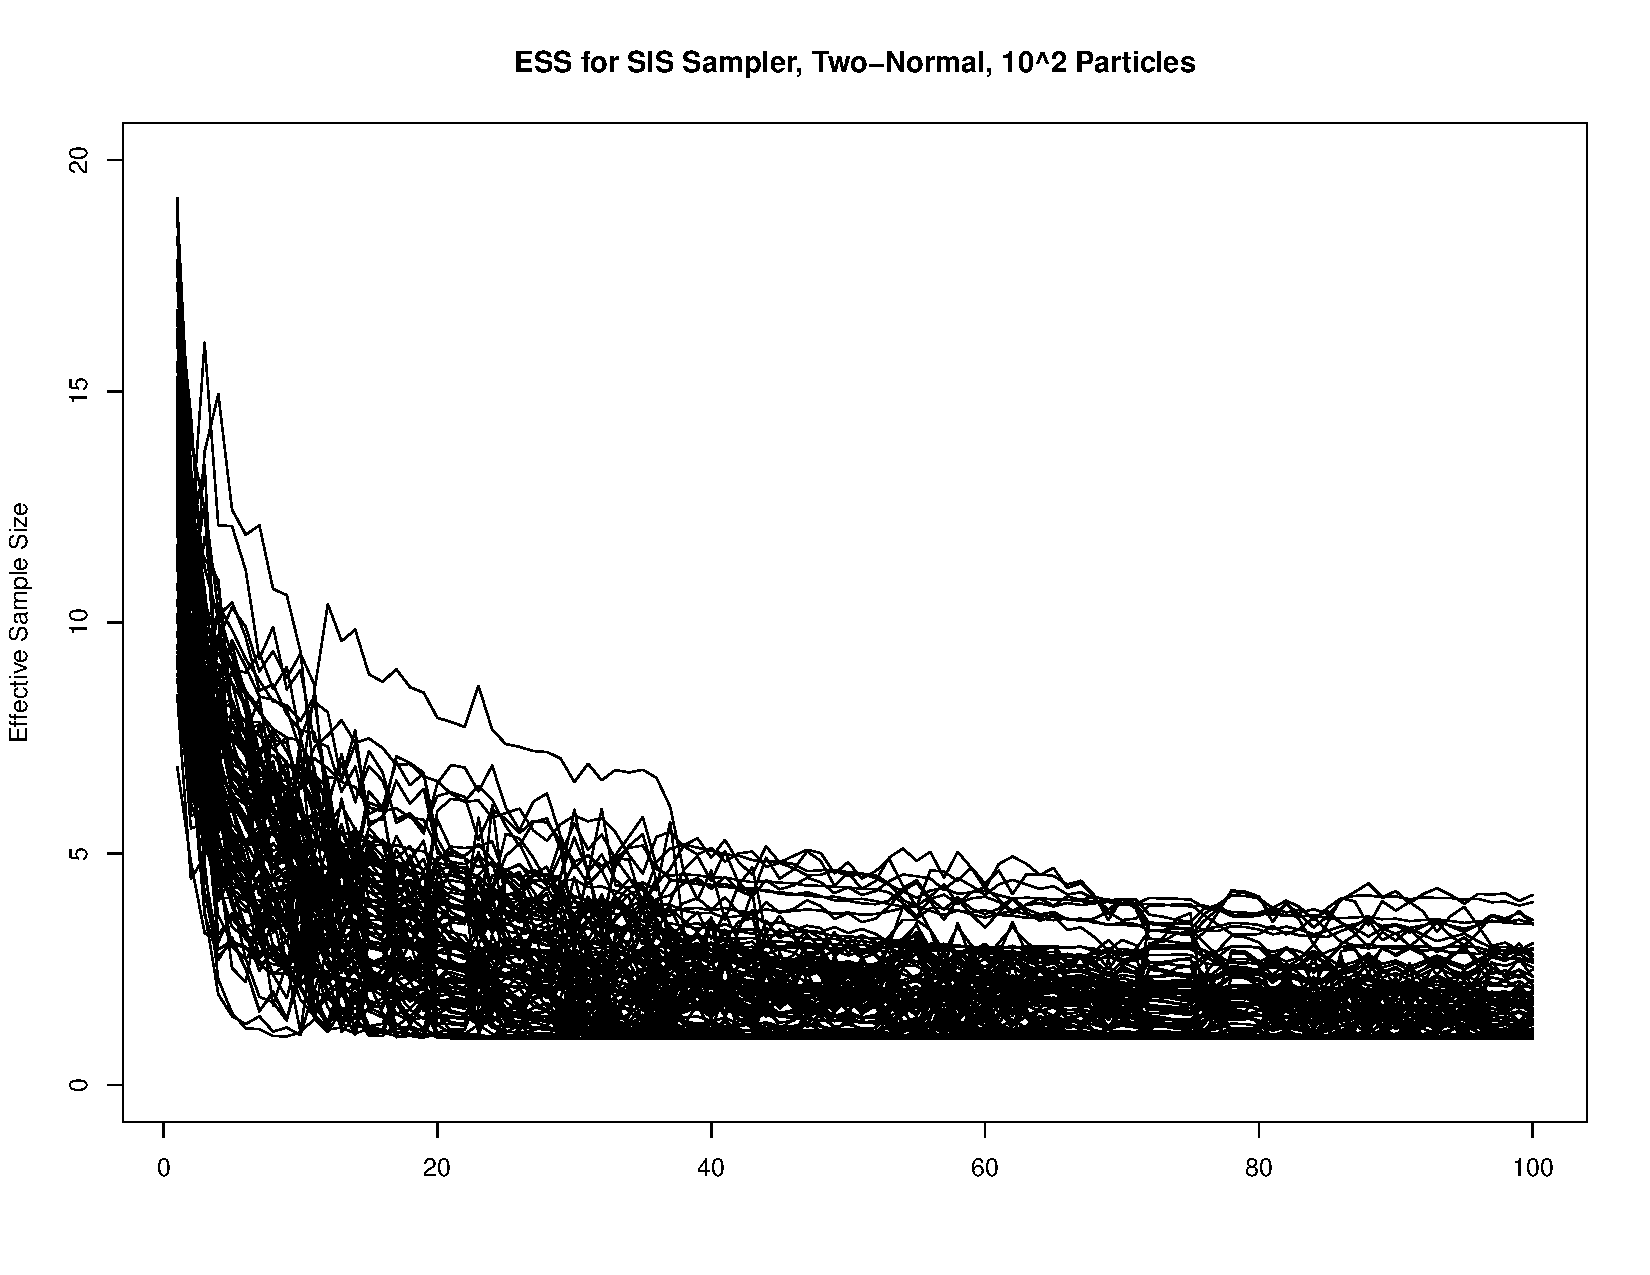
\includegraphics[width=\textwidth]{Mix_10e2_f01_ESS.pdf}
\caption{Effective sample size (ESS) for two-Normal mixture model using the SIS sampler. As noted in the text, the ESS falls to $< 5$ very quickly, and to $1$ in most cases.}
\end{figure}

On the other hand, both the NS-det and NS-rand algorithms perform well in this example, hewing closely to the MC estimate with low variance. {\sc Table 3} details the results; in particular, there is an order-of-magnitude difference between the RMSE values of the NS-det/rand algorithms and SIS algorithms in this example. Computational costs induced the use of only $N = 100$ particles for this example.

\begin{table}[b]\centering
\caption{Comparison of IS, NS-det, and NS-rand samplers in mean and RMSE for computing $\log Z$ for $N = 100, 1000$ particles with $f = 0.01$. The ``exact" MC log-evidence value was $\log Z = -338.715$. Due to computational costs, 100 simulations were run for $N = 100$ particles but only 50 for $N = 1000$ particles.}
\begin{tabular}{c|c|c|c|c|c|c}
N & IS & NS-det & NS-rand & IS RMSE & NS-det RMSE & NS-rand RMSE \\\hline
100 & -340.210 & -338.708 & -338.695 & 4.476 & 0.411 & 0.395\\
1000 & -338.725 &  -338.711 & -338.703 & 0.275 & 0.0663 & 0.0659\\ 

\end{tabular}\\
\end{table}

\begin{figure}
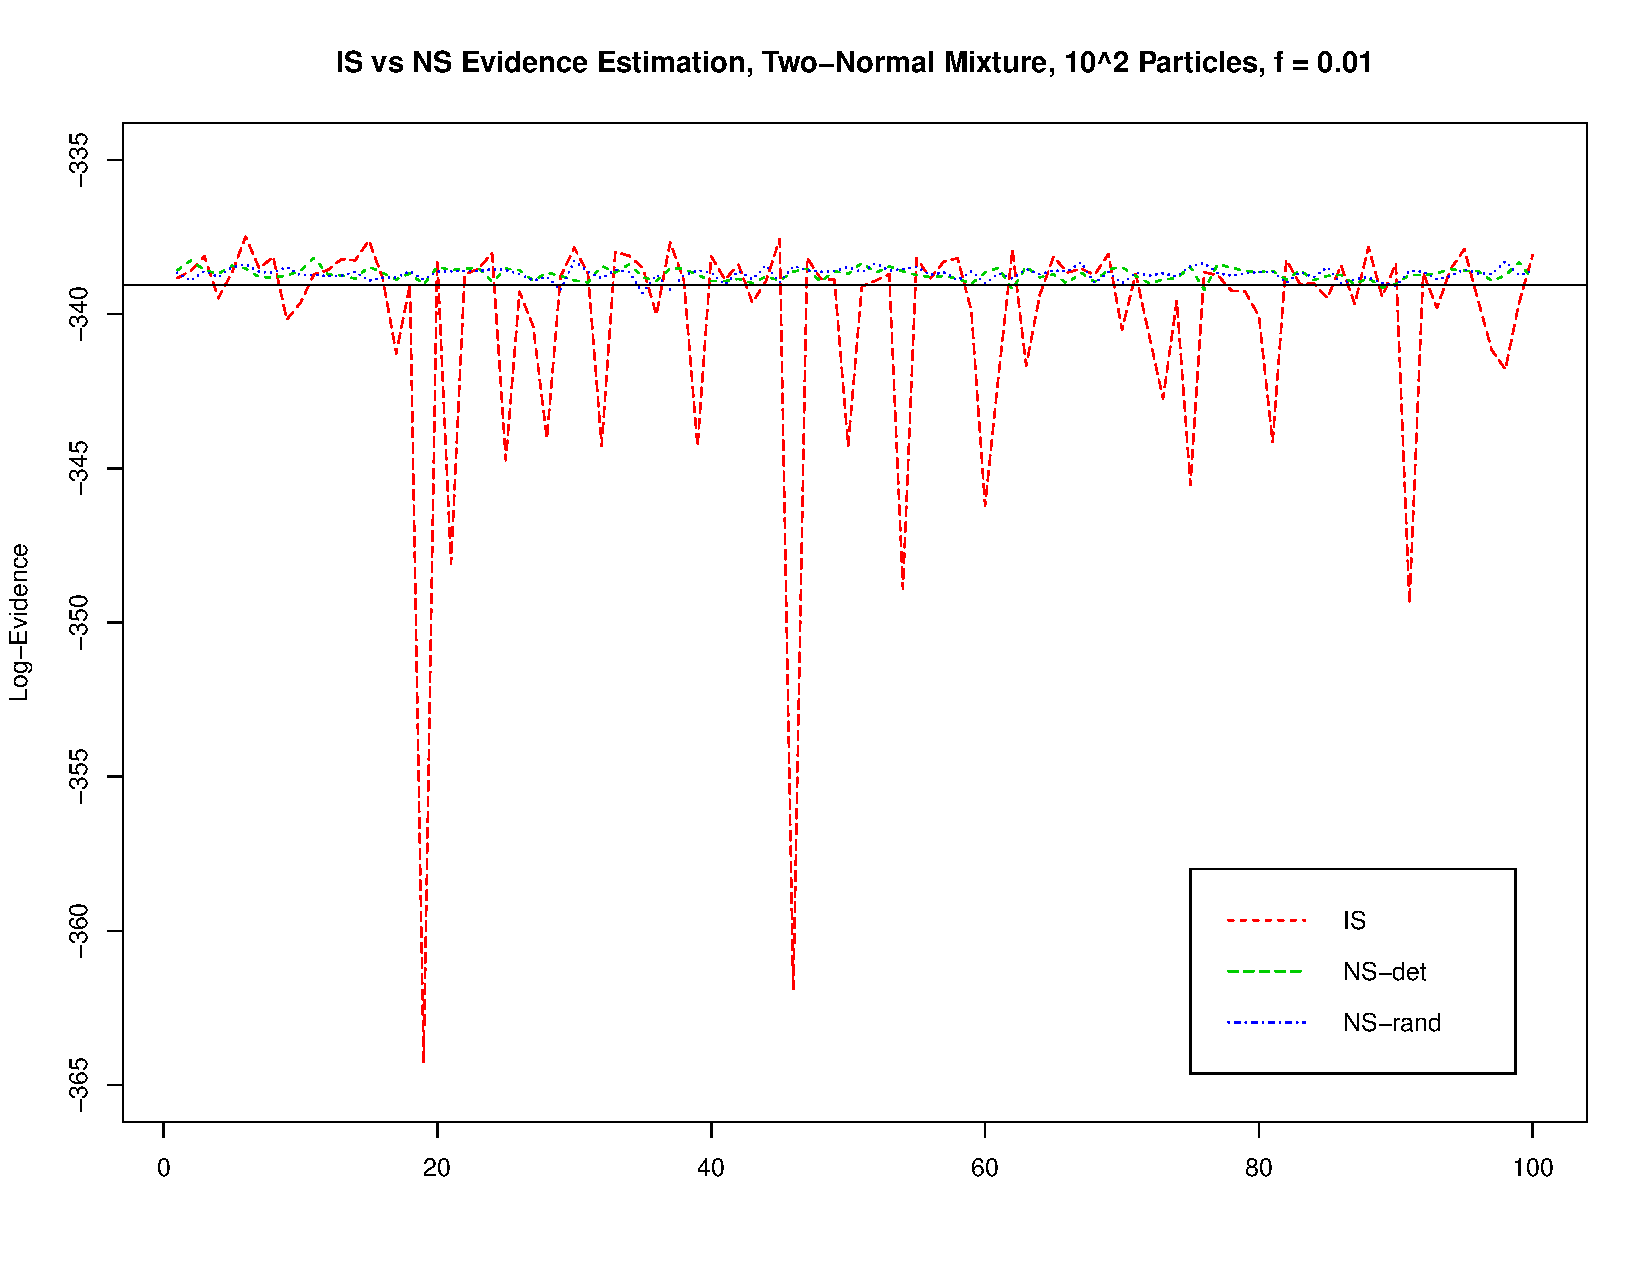
\includegraphics[width=\textwidth]{Mix_10e2_f01.pdf}
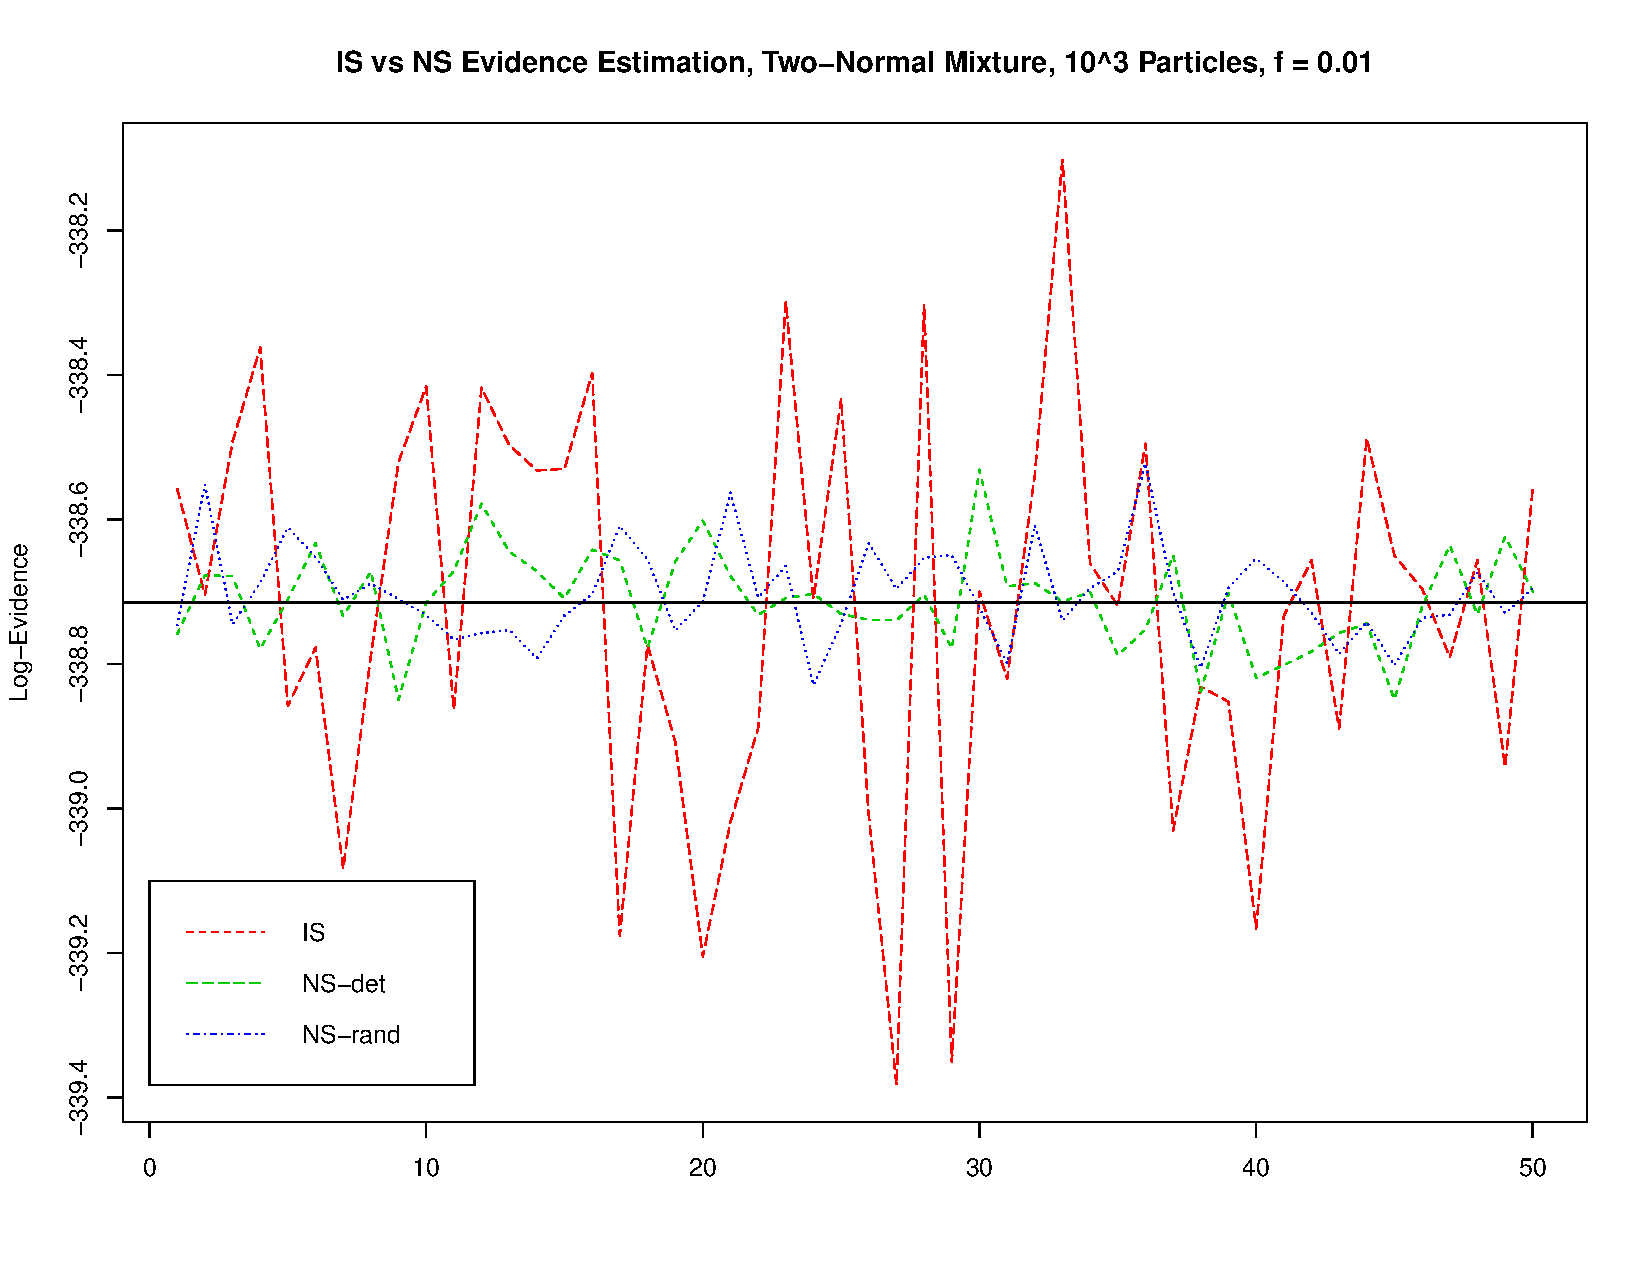
\includegraphics[width=\textwidth]{Mix_10e3_f01.pdf}
\caption{Comparison of log-evidence estimates for a two-Normal mixture model with unknown means and known variances, using the SIS, NS-det, and NS-rand samplers.}
\end{figure}

\section{Gamma-Poisson Conjugate Model}

\section{Beta-Binomial Conjugate Model}

\begin{thebibliography}{100}

\bibitem{skilling06}
Skilling, J. (2006), Nested Sampling for Bayesian Computations. {\em Proc. Valencia / ISBA 8th World Meeting on Bayesian Statistics.}
 
\bibitem{feroz14}
Feroz, F., M. P. Hobson, E. Cameron, and A. N. Pettitt (2014), Importance Nested Sampling and the MultiNest Algorithm. {\em arXiv Preprint.}

\bibitem{chopin09}
Chopin, N. and C. P. Robert (2009), Properties of Nested Sampling. {\em Biometrika} 97 (3): 741-755.


\end{thebibliography}
\end{document}
